\documentclass[xcolor=x11names, compress]{beamer}

%% General document %%%%%%%%%%%%%%%%%%%%%%%%%%%%%%%%%%
\usepackage{graphicx}
\graphicspath{{graphics/}}

\usepackage{tikz}
\usepackage{color}
\input{rgb}

\definecolor{capri}{rgb}{0,.75,1}
\definecolor{coral}{rgb}{1,.2,.2}

\newcommand{\hltyellow}[1]{\colorbox{yellow}{$\displaystyle #1$}}
\newcommand{\hltblue}[1]{\colorbox{capri}{$\displaystyle #1$}}
\newcommand{\hltred}[1]{\colorbox{coral}{$\displaystyle #1$}}
\newcommand{\hltgreen}[1]{\colorbox{green}{$\displaystyle #1$}}

\usepackage{hyperref}

\usepackage{ulem}
\renewcommand<>{\sout}[1]{
  \only#2{\beameroriginal{\sout}{#1}}
  \invisible#2{#1}
}

%%%%%%%%%%%%%%%%%%%%%%%%%%%%%%%%%%%%%%%%%%%%%%%%%%%%%%

%% Beamer Layout %%%%%%%%%%%%%%%%%%%%%%%%%%%%%%%%%%
% \usetheme{Madrid}

\useoutertheme[subsection=false,shadow]{miniframes}
\useinnertheme{default}
\usefonttheme{serif}
\usepackage{palatino}

\setbeamerfont{title like}{shape=\scshape}
\setbeamerfont{frametitle}{shape=\scshape, series = \bfseries}
\setbeamertemplate{frametitle}[default][center]
\setbeamerfont{footnote}{size=\tiny}
\addtobeamertemplate{footnote}{}{\vspace{1ex}} %so that the footnotes do not overlap with navigation symbols at bottom

\setbeamercolor*{lower separation line head}{bg=DeepSkyBlue4} 
\setbeamercolor*{normal text}{fg=black,bg=white} 
\setbeamercolor*{alerted text}{fg=red} 
\setbeamercolor*{example text}{fg=black} 
\setbeamercolor*{structure}{fg=black}
 
\setbeamercolor*{palette tertiary}{fg=black,bg=black!10} 
\setbeamercolor*{palette quaternary}{fg=black,bg=black!10} 

\renewcommand{\(}{\begin{columns}}
\renewcommand{\)}{\end{columns}}
\newcommand{\<}[1]{\begin{column}{#1}}
\renewcommand{\>}{\end{column}}

\def\signed #1{{\leavevmode\unskip\nobreak\hfil\penalty50\hskip2em
  \hbox{}\nobreak\hfil(#1)%
  \parfillskip=0pt \finalhyphendemerits=0 \endgraf}}

\newsavebox\mybox
\newenvironment{aquote}[1]
  {\savebox\mybox{#1}\begin{quote}}
  {\signed{\usebox\mybox}\end{quote}}


%%%%%%%%%%%%%%%%%%%%%%%%%%%%%%%%%%%%%%%%%%%%%%%%%%%%

\begin{document}

%%%%%%%%%%%%%%%%%%%%%%%%%%%%%%%%%%%%%%%%%%%%%%%%%%%%%%
{
  \usebackgroundtemplate{\includegraphics[width=\paperwidth]{back.jpg}}
\begin{frame}[plain]

  \vspace{100pt}
  \title{\bf The metabolic basis of species interactions}

% \author{
% 	Samraat Pawar\\
% 	\vspace{5pt}
% 	\url{www.pawarlab.org}\\
% 	\vspace{5pt}
% 	{\it  Department of Life Sciences, Silwood Park Campus}\\
% Imperial College London\\
%   \vspace{5pt}
% \today
  % \centering
  % \includegraphics[height = .3in]{Imperial_Color1.pdf}
% }
 
\titlepage
\date{} 

\end{frame}
}

%%%%%%%%%%%%%%%%%%%%%%%%%%%%%%%%%%%%%%%%%%%%%%%%%%%%%%
\section{\scshape Introduction}
% \subsection{}
%%%%%%%%%%%%%%%%%%%%%%%%%%%%%%%%%%%%%%%%%%%%%%%%%%%%%%

\begin{frame}{Outline}
  \begin{itemize}\setlength{\itemindent}{0em}\itemsep12pt

    \item Introduction (Why {\it do\/} Consumers Exist?)

    \item The Role of Size

    \item The Role of Temperature

    \item Consumer-Resource Dynamics 

    \item Summary, Questions, and Readings

  \end{itemize}  

\end{frame}

%%%%%%%%%%%%%%%%%%%%%%%%%%%%%%%%%%%%%%%%%%%%%%%%%%%%%%
\begin{frame}{Consumer-Resource Interactions}

\begin{center}
  \includegraphics[width=\textwidth]{Consumer-resource.pdf}  
\end{center}

\end{frame}

%%%%%%%%%%%%%%%%%%%%%%%%%%%%%%%%%%%%%%%%%%%%%%%%%%%%%%
\begin{frame}{Consumer-Resource Interactions}

\begin{itemize}\itemsep6pt
  \item Consumers `live to eat` and `eat to live`
  \item They are `heterotrophs`: harvest energy from other organisms (e.g., Tigers) or from other {\it organic} sources (e.g., Bacteria) 
\end{itemize}

\pause
\begin{columns}[c]
  \column{0.25\textwidth}\centering
    \vspace*{\fill} \includegraphics[width=.9\textwidth]{Boltz.jpg} 
    {\tiny By Unknown author - Universit\"{a}t Wien, Public Domain, \url{https://commons.wikimedia.org/w/index.php?curid=867246}\par}\vspace*{\fill}  
  \column{0.75\textwidth}\centering
  \vspace*{\fill} 
  \begin{quote} 
  The 'struggle for existence' of living beings is not for the fundamental constituents of food ... but for the possession of the free energy obtained, chiefly by means of the green plant, from the transfer of radiant energy from the hot sun to the cold earth. \\
  \centering
    \hfill -- {\small Ludwig Boltzmann 1886, ``The Second Law of Thermodynamics''}
\end{quote}
\vspace*{\fill}
\end{columns}

\end{frame}

%%%%%%%%%%%%%%%%%%%%%%%%%%%%%%%%%%%%%%%%%%%%%%%%%%%%%%

\begin{frame}{Why {\it do} consumers exist?}

\begin{tikzpicture}
  \node (img1) {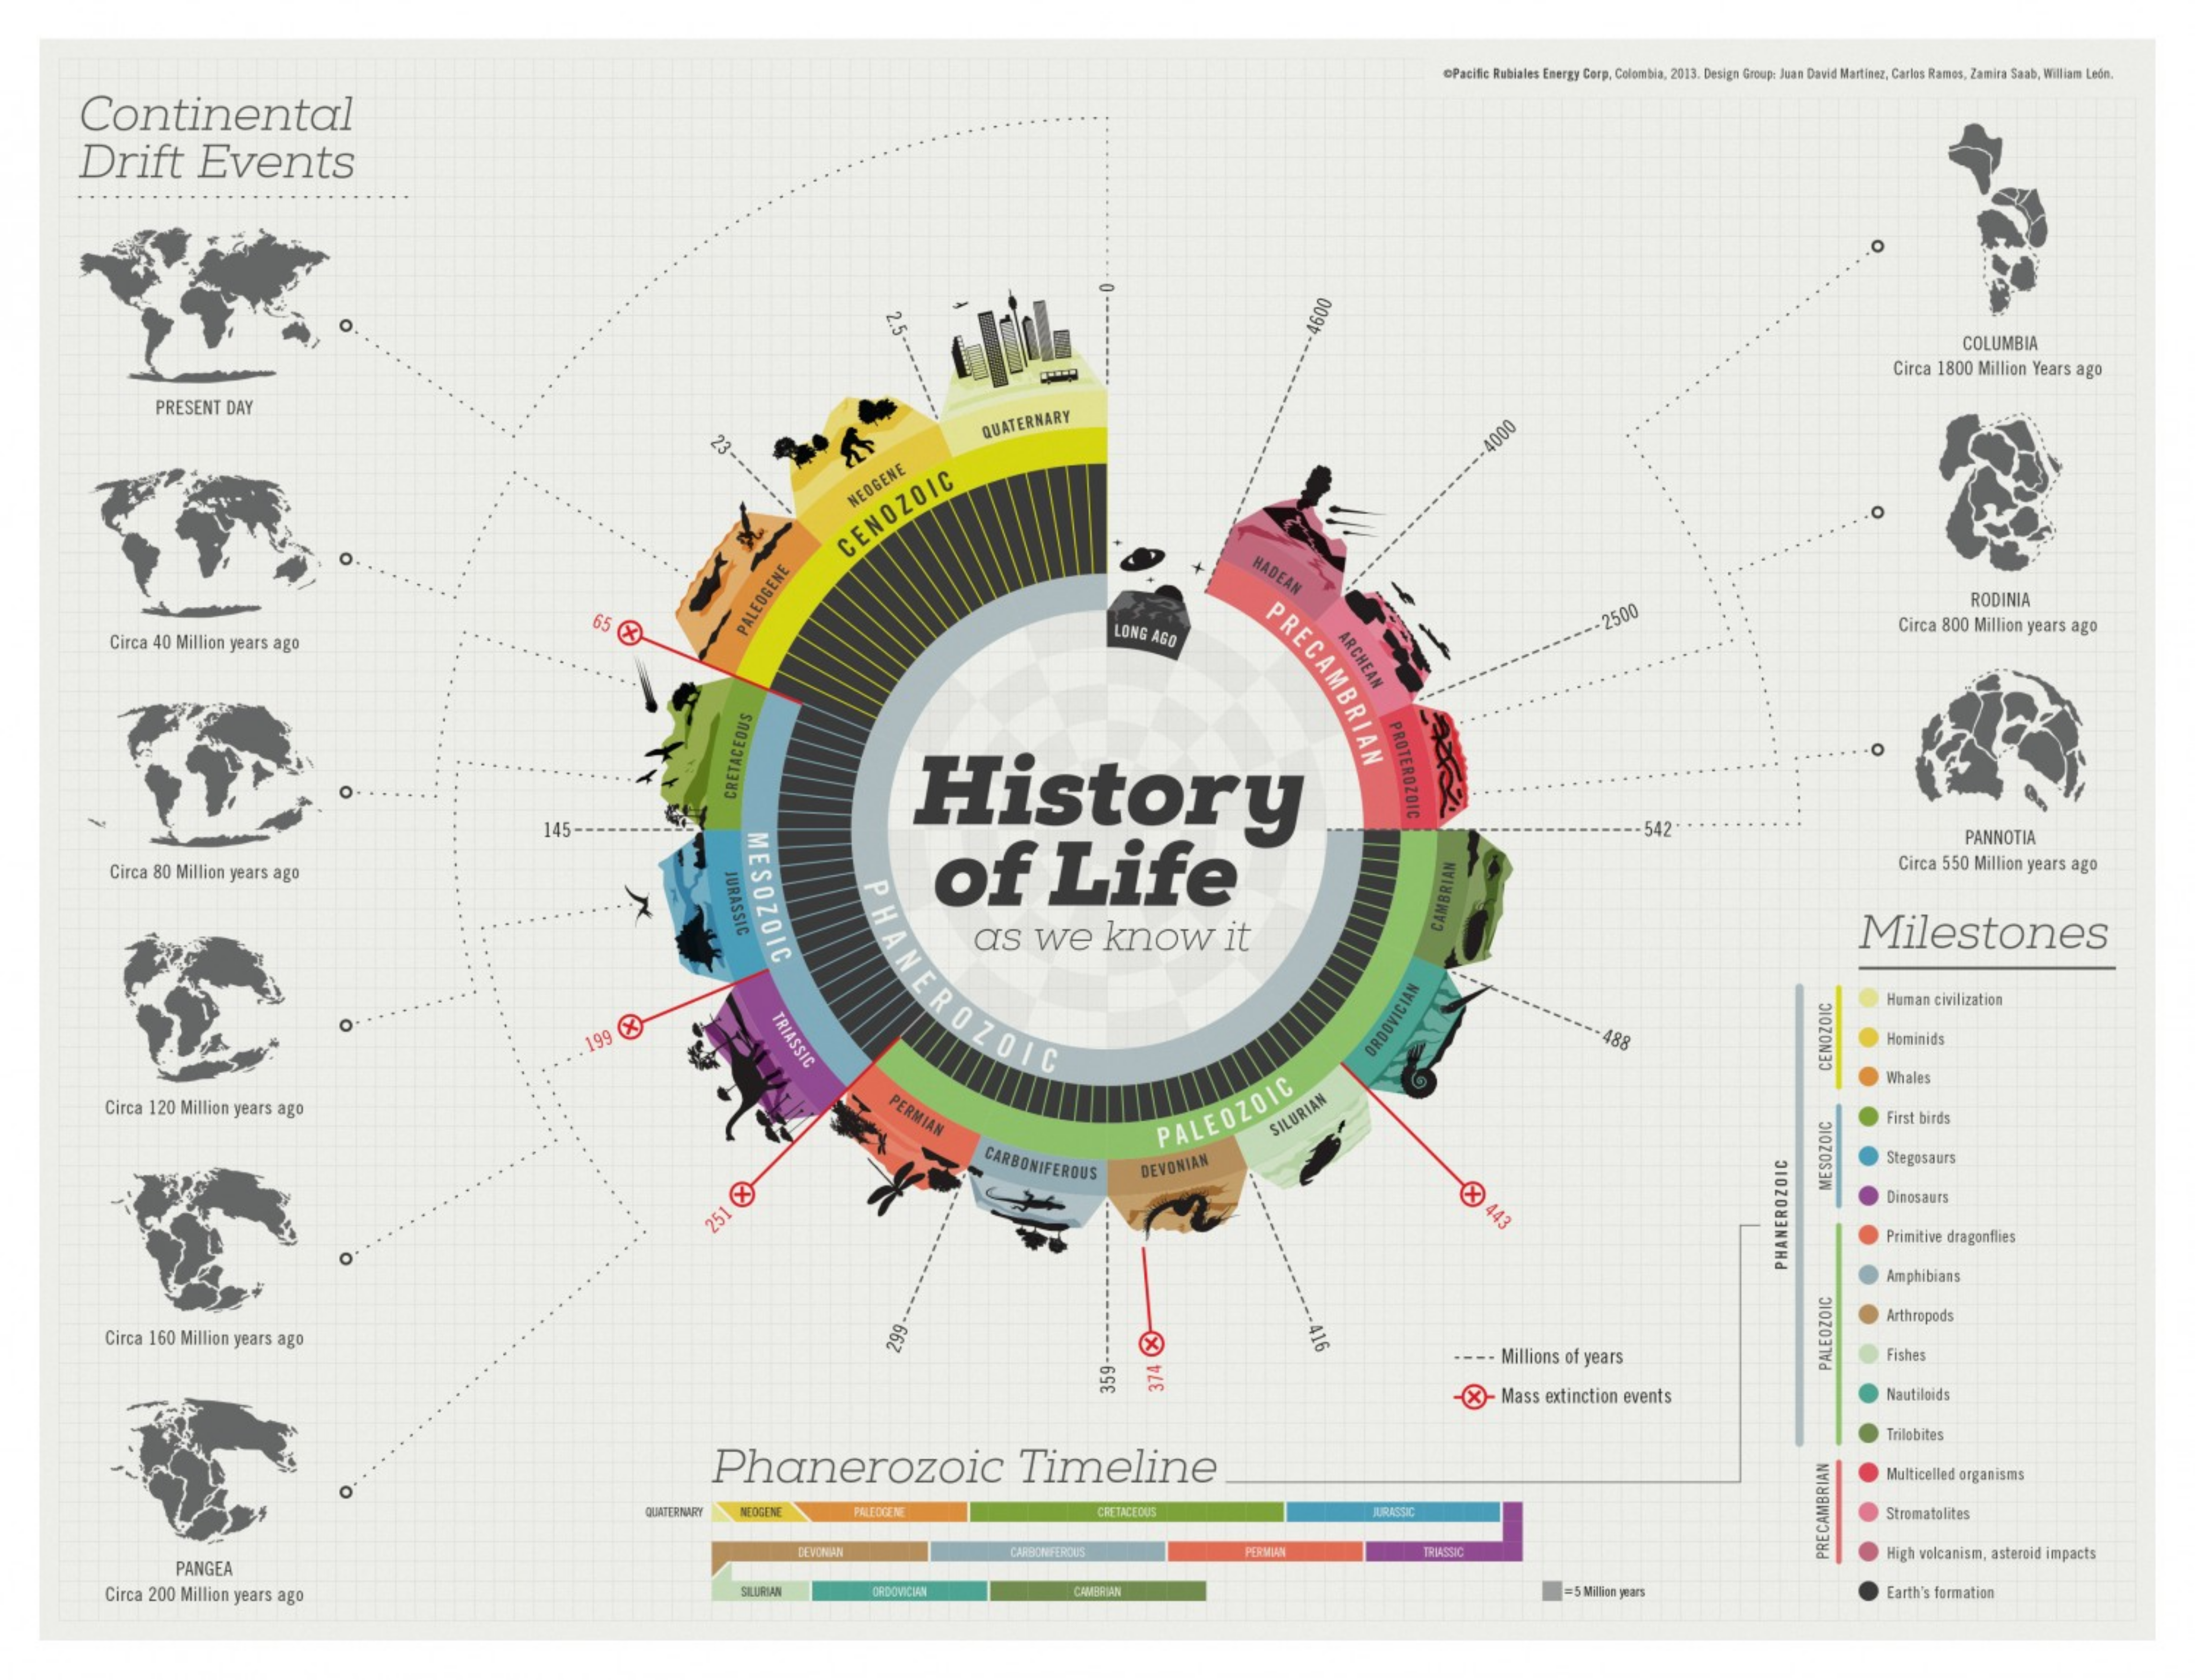
\includegraphics[width=3.9in]{History1.png}};
  \pause
  \node (img2) at (img1) {\includegraphics[width=3.9in]{History2.png}};
  \pause
  \node (img3) at (img1) {\includegraphics[width=3.9in]{History3.png}};
  \pause
  \node (img4) at (img1) {\includegraphics[width=3.9in]{History4.png}};
  \pause
  \node (img5) at (img1) {\includegraphics[width=3.9in]{History5.png}};
\end{tikzpicture}

\end{frame}

%%%%%%%%%%%%%%%%%%%%%%%%%%%%%%%%%%%%%%%%%%%%%%%%%%%%%%
\begin{frame}{A Metabolic Ecology roadmap}

  \begin{center}
    \includegraphics[width=0.8\textwidth]{Roadmap.pdf}
  \end{center}

  \vspace{6pt}
  \begin{itemize}[<+->]\setlength{\itemindent}{0em} \itemsep6pt
    \item Individual-level {\it energy use and metabolic rate\/} determines:
      \begin{itemize}\setlength{\itemindent}{0em} \itemsep6pt
        \item Interaction rates with other individuals, especially, consumption
        rates
        \item Properties of interaction networks (another lecture)
      \end{itemize}
  \end{itemize}
  
  \end{frame}
  
%%%%%%%%%%%%%%%%%%%%%%%%%%%%%%%%%%%%%%%%%%%%%%%%%%%%%%
\begin{frame}{Consumer-Resource Interactions}

  \begin{center}
    \begin{tikzpicture}
     \node (img1) {\includegraphics[width=4.2in]{Roadmap1.png}};
     \node (img2) at (img1) {\includegraphics[width=4.2in]{Roadmap2.png}};  
    \end{tikzpicture}
  \end{center}
  
  \begin{itemize}[<+->]\setlength{\itemindent}{0em}
    \item We will focus on (metabolically-constrained) consumer-resource interactions in this lecture  
  \end{itemize}
  

\end{frame}
  
%%%%%%%%%%%%%%%%%%%%%%%%%%%%%%%%%%%%%%%%%%%%%%%%%%%%%%
\section{\scshape The Role of Size}
% \subsection{}
%%%%%%%%%%%%%%%%%%%%%%%%%%%%%%%%%%%%%%%%%%%%%%%%%%%%%

%%%%%%%%%%%%%%%%%%%%%%%%%%%%%%%%%%%%%%%%%%%%%%%%%%%%%
\begin{frame}{Energy, Metabolism, and Consumption}

  \begin{itemize}[<+->]\setlength{\itemindent}{-1em} \itemsep10pt
    \item All {\it living\/} organisms must be at energy balance:\\
    \begin{itemize}
      \item Energy Consumed = Energy Used (for Maintenance + Growth + Movement)
      \item Different individuals and organisms invest energy to different degrees in Maintenance vs. Growth vs. Movement 
    \end{itemize}
    \item That is, consumption rate must keep up with metabolic rate (energy use)
    \item And if you want to do anything other than maintain yourself, you need to consume faster than your metabolic rate
    \item That is, you need to {\it invest energy} to {\it get energy} (find food)
    \item This is where body size plays a big role 
  \end{itemize}
\end{frame}

%%%%%%%%%%%%%%%%%%%%%%%%%%%%%%%%%%%%%%%%%%%%%%%%%%%%%%

\begin{frame}{Size and metabolic needs}

  \begin{itemize}[<+->]\itemsep3pt
    \item (Resting) metabolic rate ($B$) increases with body size ($M$) 
    \vspace{6pt}
    \begin{columns}[c]
	    \column{0.45\textwidth}\centering
        \includegraphics[width=\textwidth]{MetabScaling.jpg}\\ 
	    \column{0.55\textwidth}\centering
	      \includegraphics[width=.9\textwidth]{Kleiber1947.jpg}
    \end{columns}
    \item \onslide<5-> Metabolic rate increases with size as a power-law\footnotemark: $B = B_0 M^b$
    \item Therefore, larger organisms also need to {\it consume} more energy 
  \end{itemize}

  \only<5->{\footnotetext{ Review lecture on Energy and Metabolism }}

\end{frame}

%%%%%%%%%%%%%%%%%%%%%%%%%%%%%%%%%%%%%%%%%%%%%%%%%%%%%%
\begin{frame}{Size and consumer-resource interactions}

  \begin{itemize}[<+->]\setlength{\itemindent}{0em}\itemsep4pt
      \item Size also affects biomechanics---how an organism interacts with the physical environment---, and movement 
      \vspace{2pt}
    \begin{columns}[c]
      \column{0.25\textwidth}\centering
        \vspace*{\fill} 
        \includegraphics[width=.6\linewidth]{Haldane.jpg}\\
        {\tiny Public Domain, \url{https://commons.wikimedia.org/w/index.php?curid=5056739}\par} 
        \vspace*{\fill}
      \column{0.75\textwidth}\centering
      \vspace*{\fill} 
      \begin{quote} 
        You can drop a mouse down a thousand-yard mine shaft; and, on 
        arriving at the bottom, it gets a slight shock and walks away, 
        provided that the ground is fairly soft. A rat is killed, a man is 
        broken, a horse splashes. \\
        \centering
        \hfill -- {\small Haldane 1926, ``On being the right size''}
        \end{quote}
      \vspace*{\fill}
    \end{columns}
  
    \item Watch: \small \url{https://www.youtube.com/watch?v=f7KSfjv4Oq0} 

    \item Therefore size also affects consumer-resource interaction, and consumption rate
  
  \end{itemize}
  
  \end{frame}
%%%%%%%%%%%%%%%%%%%%%%%%%%%%%%%%%%%%%%%%%%%%%%%%%%%%%%
\begin{frame}{Size and consumer-resource interactions}

  \begin{itemize}[<+->]\setlength{\itemindent}{-1em}
    \item Interaction rates do not always match metabolic needs (biomechanical limitations get in the way)
    \item Because consumer-resource interaction rates depend on multiple factors other than metabolic rate:
    \begin{itemize}[<+->] \setlength{\itemindent}{-1em}
      \item Mode of locomotion: Walking? Swimming? Flying?
      \item Difference between consumer-resource size and thermal	physiology (e.g., endotherm vs ectotherm):
    \end{itemize}
  \pause
  \begin{columns}[c]
    \column{0.3\textwidth}\centering
      \includegraphics[width=\textwidth]{Size-ratioL.pdf}\\ {\small \it Tiny ectotherm feeding on huge resource}
    \column{0.3\textwidth}\centering
    \includegraphics[width=\textwidth]{Size-ratioS.pdf}\\
    {\small \it Huge endotherm feeding on tiny resource}
  \end{columns}
  \item How do we quantify all this?
\end{itemize}
  
  \end{frame}
  
  %%%%%%%%%%%%%%%%%%%%%%%%%%%%%%%%%%%%%%%%%%%%%%%%%%%%%%
  \begin{frame}{Dissecting consumer-resource interactions}
  
  \begin{columns}[c]
    \column{0.55\linewidth}
    \begin{itemize}
      \item Components of consumer-resource interactions determine consumption rate ($c$)
      \item They together determine the Type II  ``functional response'': $c = \frac{aR}{1+ahR}$
    \end{itemize}
    \pause
    \column{0.45\linewidth} \centering
      {\tiny The Type II Functional Response}\\
      \vspace{2pt}
      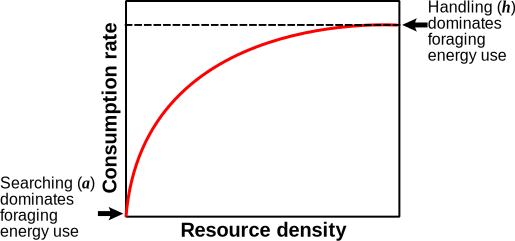
\includegraphics[width=\textwidth]{FR.pdf}\\
      {\tiny Holling, Canad. Entomol. (1959).\par}
  \end{columns}

  \vspace{16pt}

  \begin{columns}[c]
  \column{0.5\linewidth}\centering\itemsep3pt
    \includegraphics[width=\textwidth]{Components.pdf}
  \column{0.5\linewidth}	\centering
    \includegraphics[width=\textwidth]{ConsRateModel.pdf}
  \end{columns}

  \end{frame}
  
  %%%%%%%%%%%%%%%%%%%%%%%%%%%%%%%%%%%%%%%%%%%%%%%%%%%%%%
  \begin{frame}{Predicting consumer-resource interactions}

  \begin{itemize}[<+->] \setlength{\itemindent}{-1em}
    \item The key components of species interactions all {\it scale} with size:\par 
    \begin{itemize}
      \item Consumer (and resource) Velocity and Detection distance scale positively with consumer size
      \item Handling time decreases with size
      \item Consumer-resource size-difference also matters
    \end{itemize}
    \item Therefore, some key theoretical predictions emerge:\par
    \begin{columns}
      \column{.65\linewidth}\centering
        \begin{itemize}\setlength{\itemindent}{0em} \itemsep2pt
          \item Consumption rate scales positively with size 
          \item \it Consumption rate increases with (euclidean) dimensionality of interaction
          \item The scaling of consumption rate with size becomes steeper with dimensionality
      \end{itemize} 
      \column{.35\linewidth} \centering
      \includegraphics[width=\textwidth]{Dimensionality.pdf}
  \end{columns}
  \item Interaction components also depend on temperature (coming up next)
\end{itemize}

\end{frame}
  
%%%%%%%%%%%%%%%%%%%%%%%%%%%%%%%%%%%%%%%%%%%%%%%%%%%%%%
\begin{frame}{Predicting consumer-resource interactions}

\begin{center}
  {\tiny Pawar et al. Nature 2012}
\end{center}

\begin{columns}
  \column{.55\textwidth} \centering
    \includegraphics[width=\textwidth]{DimRes1.pdf}
  \column{.45\textwidth} \centering
    \includegraphics[width=\textwidth]{DimTable.pdf}
    \begin{itemize}\setlength{\itemindent}{-1em}
       \item 3$D$ consumption rates scale much more steeply with consumer size than $2D$
       \item 3$D$ consumption rate $10\times$ higher at intercept (1 kg organism)
    \end{itemize}
\end{columns}

\end{frame}
 
%%%%%%%%%%%%%%%%%%%%%%%%%%%%%%%%%%%%%%%%%%%%%%%%%%%%%%
\begin{frame}{Consumer-Resource interactions have different dimensionalities}

  \begin{center}
    \includegraphics[width=\textwidth]{Consumer-resource.pdf}  
  \end{center}
  
  \end{frame} 

  %%%%%%%%%%%%%%%%%%%%%%%%%%%%%%%%%%%%%%%%%%%%%%%%%%%%%%
\begin{frame}[plain]{}
  \begin{center}
    \includegraphics[height = 3.6in]{SeaLion.pdf}
  \end{center}
  \end{frame}
  
  %%%%%%%%%%%%%%%%%%%%%%%%%%%%%%%%%%%%%%%%%%%%%%%%%%%%%
  \begin{frame}{What about whales?!}
  
    \begin{itemize}[<+->]\setlength{\itemindent}{0em} \itemsep3pt 
       \item Recall Kleiber's (1947) plot: \\
      \begin{center}
        \includegraphics[width=.6\textwidth]{Kleiber1947.jpg}
      \end{center}
      \item {\bf Note the whale ($[\cdot]$)!} (there are more data on this now)
      \item Perhaps we have explained why whales have 
      higher-than-expected metabolic rates  --- \it because they forage in $3D$
    \end{itemize}
  
  \end{frame}

%%%%%%%%%%%%%%%%%%%%%%%%%%%%%%%%%%%%%%%%%%%%%%%%%%%%%%
\section{\scshape The Role of Temperature}
%%%%%%%%%%%%%%%%%%%%%%%%%%%%%%%%%%%%%%%%%%%%%%%%%%%%%%

%%%%%%%%%%%%%%%%%%%%%%%%%%%%%%%%%%%%%%%%%%%%%%%%%%%%%%
\begin{frame}{The importance of temperature}

  \begin{center}
    \includegraphics[width=.8\textwidth]{AMT.jpg}\\
      {\tiny CC BY-SA 3.0, \url{https://commons.wikimedia.org/w/index.php?curid=3558400}\par}
   \end{center}
    
  \end{frame}
  
  %%%%%%%%%%%%%%%%%%%%%%%%%%%%%%%%%%%%%%%%%%%%%%%%%%%%%%
  \begin{frame}{The importance of temperature}
  
    \begin{center}
      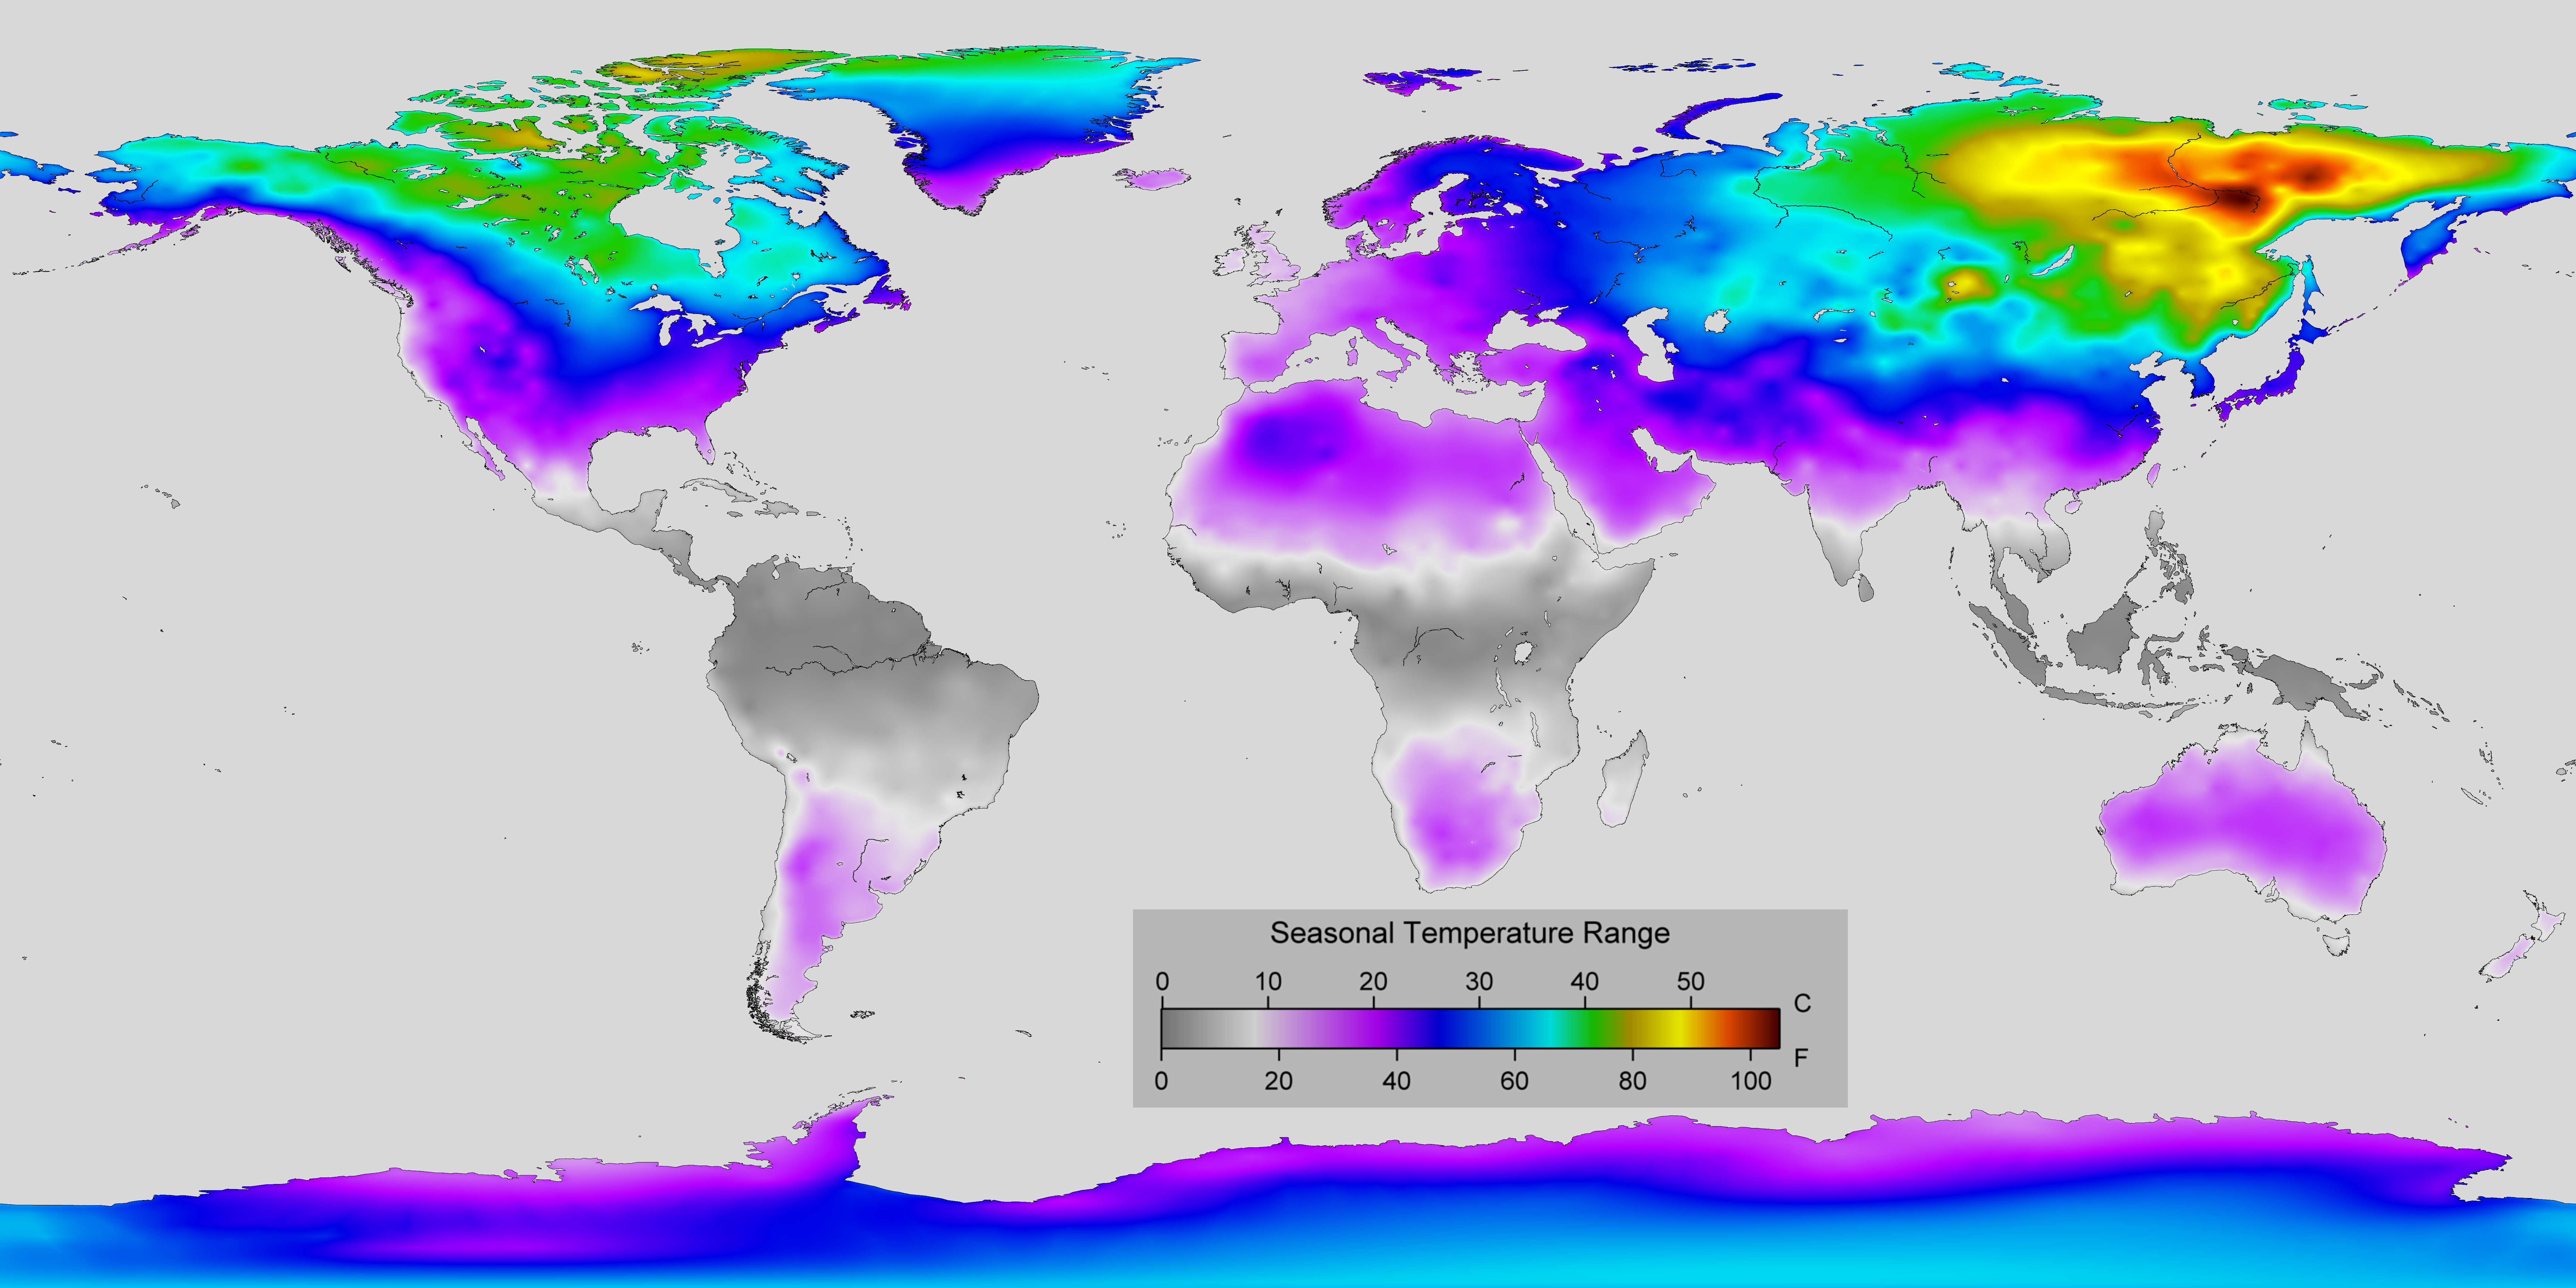
\includegraphics[width=\linewidth]{AVT.png}\\
        % {\tiny CC BY-SA 3.0, \url{https://commons.wikimedia.org/w/index.php?curid=3558400}\par}
     \end{center}
      
    \end{frame}
    
%%%%%%%%%%%%%%%%%%%%%%%%%%%%%%%%%%%%%%%%%%%%%%%%%%%%%%
\begin{frame}{Temperature and consumer-resource interactions}
  
\begin{itemize}[<+->]\setlength{\itemindent}{-1em}
    \item Components of species interactions depend on temperature (following the Boltzmann-Arrhenius response)\footnotemark:        
      \begin{itemize}\setlength{\itemindent}{-1em}
        \item Velocity of consumer (and resource) increase with temperature 
        \item Handling time decreases with temperature
      \end{itemize}
    \begin{center}
      \includegraphics[width=.45\textwidth]{Components.pdf}
    \end{center}
    \item Therefore, consumption rate increases with temperature (as does metabolic rate)
\end{itemize}

\footnotetext{Review Energy and Metabolism Lecture}
  \end{frame}

%%%%%%%%%%%%%%%%%%%%%%%%%%%%%%%%%%%%%%%%%%%%%%%%%%%%%%
\begin{frame}{Temperature and consumer-resource interactions}

\begin{itemize}[<+->]\setlength{\itemindent}{-1em}
    \item Consumer-resource interaction (and consumption) also depend on {\it physiological ``mismatches''} between the consumer and resource traits (e.g., body velocity)
    \begin{center}
      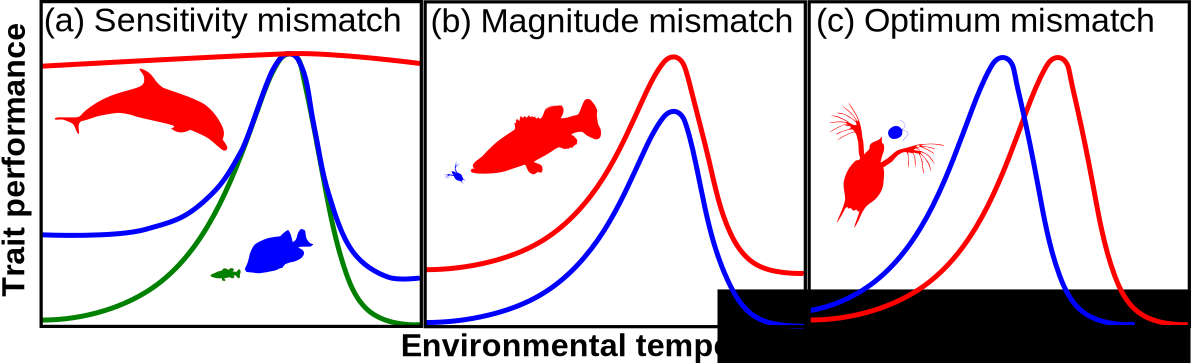
\includegraphics[width=.7\textwidth]{Mismatch.pdf}
    \end{center}          
    \item For example, 
      \begin{itemize}\setlength{\itemindent}{-1em}
        \item Panel (a): an endothermic dolphin will be able to feed on a fish species over a much wider temperature range than a fish feeding on another fish
        \item Panel (c): If both species and ectothermic are adapted to the different temperatures, the prey can escape from the predator at certain temperatures 
    \end{itemize}
\end{itemize}

\end{frame}

%%%%%%%%%%%%%%%%%%%%%%%%%%%%%%%%%%%%%%%%%%%%%%%%%%%%%%
\section{\scshape Consumer-Resource Dynamics}
% \subsection{}
%%%%%%%%%%%%%%%%%%%%%%%%%%%%%%%%%%%%%%%%%%%%%%%%%%%%%%

%%%%%%%%%%%%%%%%%%%%%%%%%%%%%%%%%%%%%%%%%%%%%%%%%%%%%%
\begin{frame}{Consumer-Resource population dynamics}

\begin{itemize}[<+->] \itemsep2pt
  \item The metabolic basis of of consumer-resource interaction rate can also be used to predict population dynamics 
  \item For example, by using the Lotka-Volterra model\footnotemark :
  {\footnotesize
  \begin{align*}
      \frac{dN}{dt} &= r_m N \left(1-\frac{N}{K}\right) - a N C\\
      \frac{dC}{dt} &= e a N C - z C
    \end{align*}\par}
     \begin{itemize}
       \item $r_m$ = Resource's maximum growth rate
       \item $K$ = Resource's carrying capacity
       \item $a$ = Consumer's {\it search rate} (or ``attack coefficient'')
       \item $e$ = Consumer's biomass conversion efficiency
       \item $z$ = Consumer's mortality rate
     \end{itemize} 
  \item All these parameters can be defined to be size- and temperature- dependent
\end{itemize}

\footnotetext{You will be playing with this model in one of your practicals}
  
\end{frame}

%%%%%%%%%%%%%%%%%%%%%%%%%%%%%%%%%%%%%%%%%%%%%%%%%%%%%%
\begin{frame}{Consumer-Resource dynamics}

  \begin{itemize}[<+->] \itemsep3pt
    \item Such metabolically-constrained models can yield useful predictions:
    \vspace{4pt}
    \begin{columns}[c]
      \column{0.6\textwidth}\centering
        Data\\
        \includegraphics[width=.9\textwidth]{L-H_cycle.png}\\
        {\it \tiny source: \url{https://www.cds.caltech.edu/~murray/amwiki/images/8/8f/LHgraph.gif}\par}
      \column{0.4\textwidth}\centering
        Model\\
        \vspace{10pt}
        \includegraphics[width=\textwidth]{LV.png}
    \end{columns} 
  
    \item Population cycles are partly driven by {\it size difference} between the two species and {\it temperature variation} over time

  \item The Lotka-Volterra model with metabolic constraints can also predict Damuth's law\footnotemark
  
\end{itemize}
  \footnotetext{Review Lecture on Energy and Metabolism}
\end{frame}

%%%%%%%%%%%%%%%%%%%%%%%%%%%%%%%%%%%%%%%%%%%%%%%%%%%%%%
\begin{frame}{Consumer-Resource dynamics}

  \begin{itemize}[<+->] \itemsep6pt
     \item Play the EcoBuilder game to see how such metabolically-informed consumer-resource models work 
  \end{itemize}

  \begin{columns}[c]
    \column{0.3\textwidth}\centering
      \includegraphics[width=.8\textwidth]{logo.pdf}\\
      \includegraphics[width=\textwidth]{device.png}
    \column{0.7\textwidth}\centering
      \begin{itemize}[<+->] \itemsep8pt
        \item Play: \small \url{https://ecobuildergame.org} (can also play in web browser: \url{https://ecobuildergame.org/Beta/}
        \item Try out the {\it Learning World}, starting with Tutorial I and II, and upto Level 4 atleast (we will revisit this game in the next Lecture)
    \end{itemize}
  \end{columns} 


\end{frame}
  

%%%%%%%%%%%%%%%%%%%%%%%%%%%%%%%%%%%%%%%%%%%%%%%%%%%%%%
\section{\scshape Summary}
% \subsection{}
   
  %%%%%%%%%%%%%%%%%%%%%%%%%%%%%%%%%%%%%%%%%%%%%%%%%%%%%%
  \begin{frame}{Summary}
  
    \begin{itemize}[<+->] \setlength{\itemindent}{0em} \itemsep10pt
  
      \item Metabolic rate and biomechanics drive
      species consumer-resource interactions, and therefore consumption rate (through the functional response)
  
      \item Consumer size, consumer-resource size difference, and interaction dimensionality influences consumer-resource interaction (and consumption) rate  
  
      \item Mismatches between species' thermal physiologies also determine
      consumer-resource interaction (and consumption) rate

      \item Consumer-resource population dynamics depend on the metabolic properties of the species (and environmental factors like dimensionality)

    \end{itemize}
  
  \end{frame}  

%%%%%%%%%%%%%%%%%%%%%%%%%%%%%%%%%%%%%%%%%%%%%%%%%%%%%%
\begin{frame}{Discussion Questions}

  \begin{enumerate}\setlength{\itemindent}{-2em}\itemsep2pt
  
    \item What are the main advantages of a consumer (heterotrophic) lifestyle  compared to an producer (autotrophic) one? What are the disadvantages? 

    \item Which is the most common and diverse organisms on planet earth\footnotemark? Why? Think in terms of what type of consumer they are, and what their size is.
        
    \item What did you learn about the role of body size in the coexistence of consumers and resources from the EcoBuilder game? What is the largest consumer on Earth? What is the smallest? In what respects is their ``struggle for existence'' similar? In what respects is it different?

    \item Which consumer(s) on earth operate(s) at the hottest temperatures? Which operate at the coldest? How is their ``struggle for existence'' similar or different?

  \end{enumerate}

  \footnotetext{See Bar-On et al, ``The Biomass Distribution on Earth'' PNAS 2018}

\end{frame}

  
  %%%%%%%%%%%%%%%%%%%%%%%%%%%%%%%%%%%%%%%%%%%%%%%%%%%%%%
  \begin{frame}{Readings}
  
  \begin{enumerate}\setlength{\itemindent}{-2em}\itemsep3pt
  
    \item Holling, C. S. Some Characteristics of Simple Types of Predation and Parasitism. Can. Entomol. 91, 385--398 (1959)
    
    \item Pawar, S., Dell, A. I. \& Savage, V. M. Dimensionality of consumer search space drives trophic interaction strengths. Nature 486, 485--489 (2012).
  
  \item DeLong, J. P. \& Vasseur, D. A. A dynamic explanation of size-density scaling in carnivores. Ecology 93, 470--476 (2012).

  \item Dell, A. I., Pawar, S. \& Savage, V. M. Temperature dependence of trophic interactions are driven by asymmetry of species responses and foraging strategy. Journal of Animal Ecology 83, 70--84 (2014).
  
  \item Grady, J. M. et al. Metabolic asymmetry and the global diversity of marine predators. Science. 363, (2019).
    
  \end{enumerate}
  
\end{frame}


\end{document}
